%%
%% Final paper - PPC 2026/27 (AI-written draft from the measured/v3 data and
%% decision records, for the author's review; see the Use of AI paragraph).
%% Based on the DI/FCUL ACM template used by the proposal and the pilot report.
%% Every number comes from data/tables/*-v3 or from the record named in
%% paper/README.md.
%%
\documentclass[sigplan]{acmart}
\settopmatter{printacmref=false}
\renewcommand\footnotetextcopyrightpermission[1]{}
\usepackage[english]{babel}
\usepackage{booktabs}
\usepackage{enumitem}
\usepackage{graphicx}

\begin{document}
\raggedbottom
\setlength{\emergencystretch}{2em}

\title{Scalability of Parallel Code in WebAssembly in the Browser vs.\ Native}

\author{David Coimbra - fc68024}
\affiliation{%
 \institution{
  Programação Paralela e Concorrente \\
  Mestrado em Engenharia Informática \\
  Faculdade de Ciências, Universidade de Lisboa}
 \country{Portugal}
 }
\email{fc68024@alunos.fc.ul.pt}

\begin{abstract}
We measure whether the same parallel Rust/Rayon code scales the same way
natively and as WebAssembly (WASM) with threads in Chrome and Firefox. On 8
dedicated performance cores of an i9-14900KF we ran 5310 independent runs of
an image filter (no synchronization) and of an image histogram with shared
atomic counters or share-nothing local ones, its updates concentrated on 1
to 256 counters. With enough work per parallel region, WASM threads scale
like native code: at 8 threads Chrome's filter speedup is 0.996 times
native's (99.5\% CI [0.987, 1.004]) and Firefox's 1.055 times [1.034,
1.072], at 1.17 to 1.36 times the native time, a factor that does not grow
with the threads. Hardware counters and SIMD variants are consistent with a
filter limited by memory at 8 threads, where Firefox's slower loop loses
less. Relative to the local control, sharing counters costs Chrome up to
2.26 times what it costs natively, but most of that is there with one
thread (1.89): it is the code V8 emits for an atomic add, a
compare-and-swap loop where LLVM and SpiderMonkey emit one locked add.
Threads add 1.2 to 1.4 times when the updates fall on 16 counters or fewer
and reverse the effect (0.42) over 256, for a reason we do not show; in
Firefox they add nothing. Swapping V8's compiler removes the one-thread
penalty, and a native program with the loop reproduces it. We also report
the pitfalls of browser benchmarking that we had to control.
\end{abstract}

\keywords{WebAssembly, multithreading, scalability, synchronization, atomics, performance evaluation}

\maketitle
\pagestyle{plain}

\section{Introduction}

Heavy work increasingly runs on the web client (image and video processing,
documents, visualization, machine learning). WebAssembly~\cite{haas2017}
with threads~\cite{watt2019} makes it possible to parallelize that work in
the browser, but it is not known whether it scales like the same code
natively, or whether thread synchronization widens the gap. We ask:

\begin{description}[nosep,leftmargin=2.5em]
  \item[RQ1] How do relative speedup and efficiency of the same parallel
  code evolve with the number of threads, natively and in WASM in the
  browser?
  \item[RQ2] To what extent does synchronization between threads affect the
  scalability gap between WASM and native?
\end{description}

\noindent Contributions: (i) a controlled comparison of one Rust/Rayon
source, compiled with the same compiler and flags for native and WASM, in
two browser engines, under an analysis plan fixed before the first
measurement and replicated on a corrected build; (ii) a design that
separates the cost of shared atomics from the input and from the code of
one thread, over four contention levels; (iii) explanations tested against
predictions written before each test, with what stays unexplained said;
(iv) the problems of browser benchmarking that we met and their controls.

\section{Background and Related Work}

WASM threads are Web Workers that share one linear memory. Rayon, a
work-stealing library, runs on them through \texttt{wasm-bindgen-rayon}. A
\emph{parallel region} is one Rayon parallel loop, here one pass over an
image; entering and leaving it is its \emph{fork-join}. Rust is compiled by
LLVM; a browser engine (V8 in Chrome, SpiderMonkey in Firefox) compiles the
WASM again, first with a fast \emph{baseline} compiler, then with an
\emph{optimizing} one that replaces its code. $T_N$ is the time with a pool
of $N$ threads ($T_1$ is not sequential code); relative speedup $S_N =
T_1/T_N$ compares an environment with itself, and efficiency is $S_N/N$.

Single-threaded WASM was measured 45 to 55\% slower than native on average
by Jangda et al.~\cite{jangda2019}, and Yan et al.~\cite{yan2021} showed
that compiler, flags, input and browser change WASM results; both are
single-threaded, so we pin all four and add threads. Szewczyk et
al.~\cite{szewczyk2022} found fast runtimes within 20\% of native and
bounds checks costing up to 650\%, outside browsers. S{\'a}nchez-Artigas
and Bohoyo-Bengoetxea~\cite{sanchez2025} found allocator and atomics
overheads in portable WASM multithreading outside the browser. Schweizer et
al.~\cite{schweizer2015} showed that atomic operations on x86 have similar
latency whatever their semantics and are bound by cache-line transfers, the
mechanism behind our RQ2 design. Closest to us, Kyriakou and
Tselikas~\cite{kyriakou2022} measured Rust as WASM in Chromium at 93.5\% of
the equivalent Node.js implementation single-threaded and 67.9\%
multithreaded. We add a thread sweep with native code as the reference in
two engines, synchronization as a controlled factor, inferential
statistics~\cite{georges2007,hoefler2015} and tested explanations.

\section{Methodology}

\paragraph{Platform.} An Intel i9-14900KF with 8 performance cores
(P-cores) and 16 efficiency cores (E-cores), 64~GB of RAM, Ubuntu 26.04.1
LTS (kernel 7.0.0-43, microcode 0x133). Turbo and SMT are off and the
frequency governor is \texttt{performance}, so the P-cores run at their
3.2~GHz base clock. A CPU-affinity mask confines each run to the 8 P-cores
whatever $N$ (a browser cannot pin single threads); the rest of the system
and the harness are confined to the E-cores, and desktop and background
services are stopped. In a pilot, adding the E-cores made runs at $N=8$ up
to 19\% slower.

\paragraph{Builds.} One Rust source~\cite{repo} (nightly 2026-10-03, Rayon
1.12.0, wasm-bindgen 0.2.129, wasm-bindgen-rayon 1.3.0, \texttt{lto=fat},
one codegen unit, \texttt{panic=abort}), compiled for x86-64 with SSE2 only
and for \texttt{wasm32} with \texttt{+atomics}, \texttt{+bulk-memory},
\texttt{+mutable-globals}, \texttt{+simd128} and \texttt{-Z build-std}:
both sides use 128-bit SIMD (the engines encode it with newer instructions
than SSE2). Browsers: Chrome for Testing 155.0.8059.84 and Firefox 158.0,
headless (headful within 0.3\% in a pilot), each run with a fresh profile
and no automation framework: the harness launches the binary and the page
posts its results to a local server. The study was measured on three
builds, never mixed, since code layout alone changes
timing~\cite{mytkowicz2009}. A review of the first found asymmetries of our
own (a bounds check paid by one histogram only, a final step timed in some
variants only), fixed in the second. The third, reported here and built
twice with equal digests, replicates the second, whose results were known:
it adds sequential references and gives both histograms the same
task-splitting code. It was adopted by a rule set beforehand (every planned
run valid, whatever it showed).

\paragraph{Workloads.} A $3\times3$ Gaussian filter (integer kernel,
row-parallel, no synchronization) is the RQ1 reference. The histogram of an
image has two variants with identical results: \emph{atomic}, 256 shared
\texttt{AtomicU64} counters, each padded to 128 bytes so that no two share
a cache line or the adjacent line the prefetcher fetches with it; and
\emph{local}, the share-nothing control, with counters private to each task
and merged at the end. Both split the image into tasks with the same code
and include their last step in the timed region. Allocation stays outside
it (WASM's default allocator has a global lock). Inputs are
8192$\times$8192 images of 8-bit pixels from a fixed seed; the histogram's
pixels take $k \in \{1,4,16,256\}$ distinct values uniformly, so the
updates spread over $k$ counters. A sequential version of each kernel,
without Rayon, is a reference at one thread. Every run checks a checksum of
its output, equal across environments and thread counts.

\paragraph{Runs.} One run is one fresh process (or browser launch).
Repetition has two levels~\cite{kalibera2013}: runs re-draw start-up
effects; iterations are summarized within their run,
the unit of analysis~\cite{georges2007}. An iteration is one pass over the
image, timed with the monotonic clock natively and
\texttt{performance.now()} in a worker (resolution 5~µs in Chrome, 20~µs in
Firefox). A run creates its pool of $N$ threads, times an empty parallel
call 20 times (the fork-join cost), then does $W$ warm-up iterations and 10
measured ones; its value is their median. $W$ was fixed per workload from
long pilot runs as 1.5 times the longest warm-up seen in any environment (5
for the atomic histogram, 15 to 71 elsewhere).

\paragraph{Campaign.} 3 environments $\times$ (9 configurations $\times$
$N \in \{1,2,4,6,7,8\}$ + 5 sequential references) $\times$ 30 runs = 5310
runs in one random order (seed 2026112201); the 9 configurations are the
filter and the two histograms at each $k$. No run failed or was excluded,
no checksum differed, no run had over 0.25~s of CPU time used by other
processes on the measured cores, and no median iteration was under 100
clock ticks. Three controls came from problems met in pilots. Chrome's
browser process moved itself out of the CPU mask through the desktop
session bus: the harness withholds the bus and checks every run for escaped
processes. Firefox was still starting up during short iterations (up to
32\% slower): every browser run waits 3~s first. The pinned Firefox updated
itself during a campaign: only the policy \texttt{DisableAppUpdate} stops
it, and each run's version is checked.

\paragraph{Analysis.} Fixed before the first campaign (committed on
2026-10-18) and unchanged since; the reported campaign replicates it. A
configuration's centre is the geometric mean of its 30 run values;
intervals are percentile bootstraps (each group of runs resampled
independently, 10\,000 times). The primary family has 10 contrasts at
$N=8$, 2 browsers $\times$ (filter + 4 values of $k$): for RQ1, the
filter's speedup ratio browser/native; for RQ2, $\exp(\Delta r)$ with
$\Delta r = r_{\text{browser}} - r_{\text{native}}$ and $r = \log
T_{\text{atomic}} - \log T_{\text{local}}$ at the same $k$: how many times
more sharing costs in the browser than natively. Dividing by the control
cancels what the input does to both variants alike; the control itself
depends on $k$, so both factors are reported. The ten are tested with
bootstrap $p$-values under Holm's correction (family error rate 0.05) and
shown with 99.5\% intervals ($1 - 0.05/10$, Bonferroni); everything else is
exploratory, with 95\% intervals. A rank test (Mann-Whitney
$U$~\cite{mann1947}, with Cliff's $\delta$ as effect size) was added after
the first build's results, and the plan's three sensitivity checks repeat
the contrasts with the per-run mean, the median across runs and no
exclusion rule. The explanations were tested after the main campaign; each
hypothesis, and what its test would show if it held or failed, was written
before the test ran.

\section{Results}

\begin{figure*}[t]
\centering
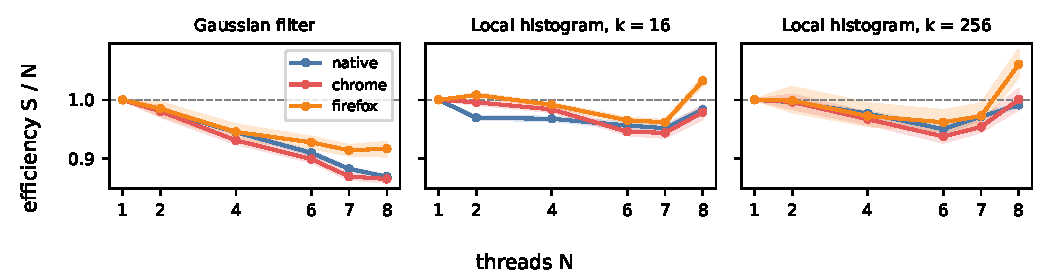
\includegraphics[width=\textwidth]{../figures/campaign-efficiency-paper.pdf}
\Description{Efficiency against thread count for the filter and the local histogram at k = 16 and k = 256, one line per environment.}
\caption{Efficiency $S_N/N$ against $N$ (geometric means of 30 runs; bands:
95\% CI; dashed: ideal).}
\label{fig:efficiency}
\end{figure*}

Runs are tight: the interquartile range is at most 2.8\% of the median for
the filter and 0.4\% for the atomic histogram at $k=256$. At $k=1$ the
atomic runs fall on several time levels 12 to 20\% apart. The ten primary
decisions hold under the three sensitivity checks and the rank test
(rejected: $|\delta| \ge 0.74$; the others $p \ge 0.10$).

\subsection{RQ1: scaling without synchronization}

Figure~\ref{fig:efficiency} shows how efficiency evolves. The filter's
falls slowly and alike in the three environments: 0.98 at $N=2$, 0.93 to
0.95 at $N=4$, and at $N=8$ 0.87 natively and in Chrome and 0.92 in Firefox
(speedups 6.96, 6.92 and 7.34). Firefox departs from native only from $N=6$
on (speedup ratios 1.02, 1.04, 1.055). Chrome is 1.2 to 1.5\% below native
at $N=4$ to 7 (exploratory) and within $-1.3$ to $+0.4$\% at $N=8$: the
primary ratio is 0.996 (99.5\% CI [0.987, 1.004], not rejected), against
Firefox's 1.055 [1.034, 1.072], rejected. The local histogram stays between
0.94 and 1.06 at every $k$ and $N$; it dips at $N=6$ and 7 everywhere and
passes 1 in Firefox at $k \ge 16$ (speedup 8.48 at $k=256$).

In absolute time WASM is slower on one thread for the filter (Chrome
1.17$\times$ native, Firefox 1.36$\times$) and for the local histogram at
$k \ge 16$ (1.23 to 1.27$\times$), and within 7\% at $k \le 4$; the ratio
does not grow with $N$ (filter at $N=8$: 1.18 and 1.29). On these workloads
WASM threads cost time, not scalability. Part of Firefox's higher speedup
is its baseline: for the filter and the local histogram a pool of one
thread takes between 7\% less and 5\% more than the sequential reference,
and against that reference the filter reaches 6.90, 6.86 and 7.15, so
Firefox's ratio to native falls from 1.055 to 1.04.

This holds for large regions. An empty parallel call at $N=8$ takes 110~µs
in Chrome and 60~µs in Firefox (three ticks of its clock) against 7.9~µs
natively (medians; the means are 164, 91 and 46~µs). That is 0.2\%
(native) to 2.9\% (Chrome) of a filter iteration here and a large share of
a small region (Section~\ref{sec:extensions}).

\subsection{RQ2: the effect of synchronization}

\begin{table}[t]
\caption{RQ2: $\exp(\Delta r)$, the atomic/local time ratio in the browser
over the same ratio natively. $N=8$: the primary contrasts, with 99.5\% CI.
$N=1$: the same with one thread (exploratory; 95\% CI within $\pm$2\%).}
\label{tab:rq2}
\footnotesize
\setlength{\tabcolsep}{3pt}
\begin{tabular}{lcccc}
\toprule
& \multicolumn{2}{c}{Chrome} & \multicolumn{2}{c}{Firefox} \\
$k$ & $N$=1 & $N$=8 & $N$=1 & $N$=8 \\
\midrule
1 & 1.89 & \textbf{2.26} [2.11, 2.41] & 1.00 & 1.01 [0.96, 1.07] \\
4 & 1.45 & \textbf{1.77} [1.75, 1.79] & 0.98 & \textbf{0.97} [0.96, 0.98] \\
16 & 1.03 & \textbf{1.43} [1.40, 1.45] & 0.79 & \textbf{0.83} [0.82, 0.84] \\
256 & 0.88 & \textbf{0.42} [0.41, 0.43] & 0.79 & \textbf{0.80} [0.78, 0.81] \\
\bottomrule
\end{tabular}

\smallskip
\footnotesize Bold: rejected by Holm ($\alpha = 0.05$, 10 contrasts).
\end{table}

\begin{figure}[t]
\centering
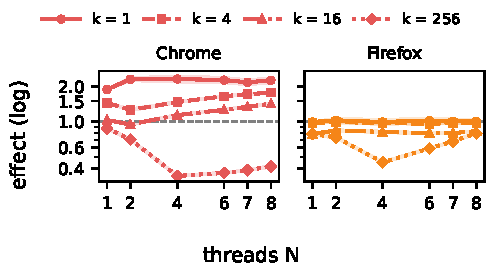
\includegraphics[width=\columnwidth]{../figures/campaign-rq2-effect.pdf}
\Description{The RQ2 effect against thread count, one panel per browser and one line per k.}
\caption{RQ2 effect $\exp(\Delta r)$ against $N$ (log scale, bands: 95\%
CI; dashed: the native cost). The value at $N=1$ is the code alone; the
change from it is what the threads add.}
\label{fig:rq2}
\end{figure}

Sharing is expensive everywhere: at $N=8$ and $k=1$ the atomic histogram
takes 44 times the control's time natively and 99 times in Chrome, and at
$k \le 16$ it is slower with 8 threads than with one (speedups 0.36 to
0.70). The question is how much more it costs in a browser
(Table~\ref{tab:rq2}, Figure~\ref{fig:rq2}). At $N=8$ it costs Chrome 2.26,
1.77 and 1.43 times what it costs natively at $k=1$, 4 and 16, and 0.42
times at $k=256$, where Chrome's atomic histogram is the only one that
speeds up (1.96 against 0.92 natively).

Most of Chrome's penalty is not contention. With one thread, where nothing
contends, the effect is already 1.89, 1.45, 1.03 and 0.88: threads multiply
it by 1.20, 1.22 and 1.38 at $k \le 16$, most at $k=16$, and by 0.47 at
$k=256$, where the whole reversal is theirs. In Firefox the threads add
nothing (1.01, 0.99, 1.06, 1.01): its effects at $k \ge 16$ exist with one
thread and come from the control, 1.19 to 1.21 times slower than native's
there while its atomic times are the native ones (0.95 to 1.03 times).
Chrome's come from the atomic variant (2.21 times native's time at $k=1$,
0.51 at $k=256$; its control is within 0.98 to 1.25).

\subsection{What explains the results}

\begin{table}[t]
\caption{The atomic histogram by increment sequence: time in ms. Engine
rows: one compiler per browser forced by flags (opt.: optimizing, base.:
baseline), geometric means of 30 runs (95\% CI: $\pm$3.5\% at $k=1$, $N=8$,
under $\pm$0.1\% elsewhere). Probe rows: a native program in which only the
increment changes (one process, median of 10 passes, pinned threads). Bold:
the compare-and-swap loop.}
\label{tab:sequence}
\footnotesize
\setlength{\tabcolsep}{2.5pt}
\begin{tabular}{llcccc}
\toprule
& & \multicolumn{2}{c}{$k=1$} & \multicolumn{2}{c}{$k=256$} \\
Code & Sequence & $N$=1 & $N$=8 & $N$=1 & $N$=8 \\
\midrule
Native & \texttt{lock inc} & 380 & 857 & 380 & 414 \\
Firefox opt. & \texttt{lock add} & 380 & 874 & 380 & 393 \\
Chrome opt. & load, \texttt{lock cmpxchg}, retry & \textbf{698} & \textbf{1823} & \textbf{412} & \textbf{210} \\
Chrome base. & \texttt{lock xadd} & 419 & 898 & 403 & 270 \\
Firefox base. & not captured & 411 & 897 & 384 & 327 \\
\midrule
Probe & \texttt{lock inc} & 380 & 976 & 380 & 415 \\
Probe & load, \texttt{lock cmpxchg}, retry & \textbf{677} & \textbf{2132} & \textbf{408} & \textbf{240} \\
\bottomrule
\end{tabular}
\end{table}

\paragraph{RQ2, the code.} We read the machine code each environment runs
for the increment of a shared counter (Table~\ref{tab:sequence}). LLVM
emits one locked add natively (\texttt{lock inc}) and SpiderMonkey another
(\texttt{lock add}): the processor adds in memory atomically. V8's
optimizing compiler emits a compare-and-swap loop: it loads the counter,
adds, and writes with \texttt{lock cmpxchg} only if the counter is
unchanged, else it retries. V8's baseline compiler emits an atomic
exchange-and-add (\texttt{lock xadd}).

\paragraph{RQ2, the compiler swapped.} A campaign of 2100 runs forced one
compiler per browser. The default configuration gives the optimizing
compiler's times (within 2.5\% in every cell), so that is what the
campaigns measure. With its baseline compiler Chrome's effect at $k=1$,
$N=8$ falls from 2.17 (in that campaign) to 1.04: the penalty follows the
compiler.

\paragraph{RQ2, the sequence alone.} A native program changed only the
increment. With the compare-and-swap loop it gives Chrome's one-thread
times within 3\% (677 and 408~ms against 698 and 412) and, at $k=256$ with
8 threads, 240~ms where the locked add takes 415 and Chrome 210. So the
sequence is enough for both directions on this CPU, which is less than
showing that nothing else contributes: the probe is one process, 14\% from
Chrome at $k=256$.

\paragraph{RQ2, the retries.} Hardware counters (\texttt{perf stat} on the
P-cores, 720 runs) count each attempt of the loop. At $k=1$, $N=8$ Chrome
makes 0.24 more per add than with one thread (95\% CI [0.23, 0.26]),
against 0.001 natively and 0.002 in Firefox, which runs the same module and
pool. Retries account for the step from one thread to eight (Chrome's
atomic time is 1.84 times native's at $N=1$ and 2.21 at $N=8$), not for the
1.84. That the loop costs more with one thread at small $k$ fits each load
waiting for the previous write to the same counter; we did not test it. Why
the loop wins at $k=256$ is not shown: there the sequences that do more
around the locked write finish sooner, the baseline compilers included (270
and 327~ms against 414), a prediction that failed in part.

\begin{table}[t]
\caption{The filter's loop alone, per pixel, from hardware counters (the
rest of a run removed by subtracting runs with 1 pass per iteration from
runs with 8; 10 runs each): cost at $N=1$ (95\% CI within $\pm$2\%) and its
change from $N=1$ to 8. LLC: last-level cache.}
\label{tab:filter}
\footnotesize
\setlength{\tabcolsep}{3pt}
\begin{tabular}{lccccc}
\toprule
& \multicolumn{2}{c}{$N=1$} & \multicolumn{3}{c}{$N=8$ over $N=1$} \\
& Instr. & Cycles & Instr. & Cycles [95\% CI] & LLC misses \\
\midrule
Native & 4.10 & 1.07 & 1.00 & 1.085 [1.076, 1.093] & 1.43 \\
Chrome & 5.52 & 1.24 & 1.00 & 1.049 [1.029, 1.071] & 1.47 \\
Firefox & 5.41 & 1.45 & 1.01 & 1.032 [1.012, 1.054] & 1.25 \\
\bottomrule
\end{tabular}
\end{table}

\paragraph{RQ1, one thread.} Both engines run about a third more
instructions per pixel than native code (Table~\ref{tab:filter}). Chrome
executes more of them per cycle and ends at 1.17 times the native cycles,
Firefox at 1.36: the time ratios of the campaign.

\paragraph{RQ1, eight threads.} From 1 to 8 threads the instructions per
pixel do not change and the cycles and cache misses rise, in the direction
predicted for a loop limited by memory and by about half the predicted
size; they rise less in Firefox than natively. Two more filter builds
change only vectorization (720 runs): with no SIMD on either side the
efficiency at $N=8$ is 0.97 to 0.98 in the three environments; with native
AVX2 it is 0.72. Across builds, the more memory one thread goes through per
second, the less 8 threads gain, and Firefox sits where its throughput puts
it. Two things do not fit. The filter is not at a ceiling: at $N=8$ it
reads 20.6~GB/s natively and the AVX2 build 25.0. And Chrome, with less
throughput than native, has the native efficiency. The cycles explain about
half of the native loss (8.5\% of 15\% more time than ideal); the rest is
time in which a core does not run the loop, far more than the fork-join,
and was not measured.

\paragraph{RQ1, above 8.} Firefox's local histogram at $k=256$ reaches 8.48
(8.12 against the sequential reference). With 8 threads its cycles per
pixel fall by 5\% and its misses in the per-core L2 cache by a quarter,
against a twentieth natively: one thread pays for misses that eight do
not, for a reason we do not know.

\subsection{Exploratory extensions}
\label{sec:extensions}

Further campaigns on the same build and protocol bound the two results
(95\% intervals, uncorrected). \emph{Atomics without sharing} (5400 runs):
with one padded table per thread nothing is shared, and the histogram
scales like the control everywhere (speedup 7.90 to 7.96), yet costs Chrome
1.85 times native at $k=1$ and 1.09 times at $k=256$ at every $N$: the
one-thread penalty again, with no contention. With eight counters per cache
line instead of one, the atomic histogram at $k=256$ slows by 1.18 times
natively, 1.25 in Firefox and 3.45 in Chrome: Chrome's advantage there
needs padding. \emph{Weak scaling}~\cite{gustafson1988} (1080 runs): the
filter keeps 0.86, 0.85 and 0.92 of its one-thread rate at $N=8$. \emph{Small regions} (4080
runs, 512$^2$ to 8192$^2$ pixels): the speedup stays above 1, but at $N=8$
the filter's efficiency falls below 0.5 under 125~µs of sequential work
natively, 396 in Chrome and 459 in Firefox, and at 4096$^2$ (about 6~ms of
sequential work) Chrome still keeps only 0.76 against native's 0.94.

\section{Discussion}

\emph{RQ1.} With enough work per parallel region, speedup and efficiency
evolve with $N$ in WASM as they do natively: the filter's efficiency falls
from 0.98 to 0.87 between 2 and 8 threads in Chrome as in native code, and
Firefox ends 5 points higher from a slower thread (4.20 against 3.25~ms at
$N=8$). WASM costs time per thread, a third more instructions per pixel
here, which divides with the work; its fork-join, several times slower,
does not. Our 17 to 36\% on one thread is below the 45 to 55\% of Jangda et
al., and our 77 to 85\% of native speed at 8 threads above the 67.9\% of
Kyriakou and Tselikas against Node.js. Amdahl's
law~\cite{amdahl1967} would read the sub-linear speedup as a serial part
(Karp and Flatt's~\cite{karp1990} inferred serial fraction is 0.021, 0.022
and 0.013 at $N=8$), but the timed region has none: it is a cost of running
in parallel. Firefox's higher speedup is not evidence that a browser runs
threads better. It is consistent with a slower loop asking less of the
memory, a reading that rests on correlations, not on an intervention on the
memory, and leaves Chrome's loss outside the loop open.

\emph{RQ2.} Sharing counters separates the engines, in two parts. One has
no threads in it: the code an engine emits for an atomic add. V8's
optimizing compiler emits a loop that makes sharing cost 1.9 times what it
costs natively at $k=1$ with a single thread; its other compiler and the
other engine do not. Memory order is not the reason: the loop has only atomic
adds, and on x86 a locked add is the same instruction for every
ordering~\cite{schweizer2015}. The other part is what RQ2 asks about: under
contention the gap widens by 1.2 to 1.4 times in Chrome at $k \le 16$,
where the loop retries, narrows to 0.42 at $k=256$ for a reason not shown,
and does not move in Firefox. A claim about ``WASM atomics'' is therefore a
claim about an engine version.

\section{Threats to Validity}

\emph{Internal.} Thread placement is left to the kernel, and at $N=8$
the browsers' own threads share the 8 cores. In
Firefox, one or two of the first three measured iterations of one
configuration (local, $k=1$, $N=8$) are 7 to 12\% slower after 71 warm-up
iterations; the run's median moves by 0.1\%. Below the shared source the
environments differ (allocator, thread start-up, clock, SIMD encoding),
which is part of what is measured. One P-core crashes programs on the
unprepared machine (likely turbo); on the prepared one it gives the right
checksum and the other cores' time.
\emph{Construct.} Synchronization here is a lock-free atomic add on padded
counters on x86-64: mutexes, condition variables and wait/notify, where a
browser differs most from an operating system, were not measured. Speedup
is relative to a pool of one thread, so absolute ratios and the sequential
reference accompany it. RQ2 is a ratio of ratios whose control depends on
$k$ (5.7 times slower at $k=1$ than at $k=256$ natively), so its factors
and its one-thread value are reported. The efficiency dip at $N=6$ and 7 is
unexplained; fixed task sizes did not remove it. \emph{External.} One
machine, P-cores only, one compiler, two pinned headless browsers, two
workloads, random inputs larger than the caches. \emph{Conclusion.}
The intervals cover run-to-run variation of one binary in one session, not
builds or boots: the previous build gave 0.990 and 1.049 for the two filter
contrasts. With 30 runs, percentile intervals at 99.5\% cover slightly
less, and the points of a curve share their $T_1$. A non-rejection is
bounded by its interval ($\pm$1\% for Chrome's filter, $\pm$6\% for
Firefox at $k=1$), not proof of equality. The explanations are exploratory:
the probe is one process, forcing a compiler changes the whole loop, and
the loop counters' comparison rules were written after a first look.

\section{Conclusion}

The same Rust/Rayon code scales in the browser as natively when each
parallel region has enough work: WASM threads cost a factor in time that
does not grow with the threads, and a slower fork-join. Where a browser
scales better, the evidence is consistent with its slower code on a loop
limited by memory. Shared atomic counters cost Chrome up to 2.26 times what
they cost natively, mostly because of the compare-and-swap loop V8's
optimizing compiler emits for an atomic add, a cost that is there with one
thread, is absent from V8's other compiler and is reproduced natively;
contention adds 1.2 to 1.4 times and reverses the effect over 256 counters,
which we reproduce but do not explain; in Firefox it adds nothing.
For developers, WASM threads pay off with coarse regions and little
sharing; for benchmarkers, a CPU mask, a fresh profile and a pinned version
do not by themselves confine, quiet and freeze a browser.

\paragraph{Use of AI} Written with Claude (Anthropic) from the project's
data and decision records.

\bibliographystyle{ACM-Reference-Format}
\bibliography{../bib/referencias}

\end{document}
